
\section{Strukturelle Induktion}
\subsection{Kantorowitsch-Bäume}
\begin{frame}
	Man kann syntaktische Ausdrücke als Kantorowitsch-Baum schreiben. \\
	Beispiel: einfacher arithmetischer Ausdruck: $3 + (a + b) \cdot (-c)$ \pause
	\begin{figure}[H]
		\centering
		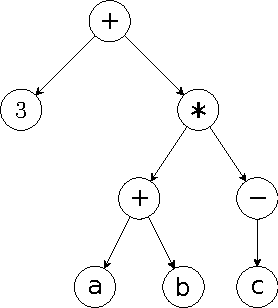
\includegraphics[width=0.4\linewidth]{struktInd/Baum.pdf}
	\end{figure}
\end{frame}

\subsection{Strukturelle Induktion}
\begin{frame}
	Aussagen mit z.B. regulären Ausdrücken, Produktionsmengen o.Ä. lassen sich am Besten über \textbf{strukturelle Induktion beweisen} \pause
	Dabei zeigt man:
	\begin{description}[<+->]
		\item[Induktionsanfang] Die Aussage stimmt für die Wurzel / jedes Atom
		\item[Induktionsvoraussetzung] Die Aussage stimmt für einen Teilbaum / einen Teilausdruck
		\item[Induktionsschluss] Die Aussage stimmt für jede Verzweigung / jeden Produktionsschritt
	\end{description}
\end{frame}

% TODO: Austauschen gegen nicht-Klausuraufgabe (Klausur März 2011)
\begin{frame}{Aufgabe}
	Die Menge $M \subset \N_0$ sei definiert durch:
	\begin{itemize}
		\item 5 und 8 liegen in $M$.
		\item Für alle $m$, $n$ gilt: Wenn $n$ und $m$ in $M$ liegen, dann ist auch $n^2 + m^2$ in $M$.
		\item Keine anderen Zahlen liegen in $M$.
	\end{itemize}
	Zeigen Sie durch strukturelle Induktion:
		$$\forall \ n \in M : n \mod 3 = 2$$
\end{frame}

\begin{frame}{Lösung}
	\begin{description}[<+->]
		\item[Induktionsanfang] $5 \mod 3 = 8 \mod 3 = 2$
		\item[Induktionsvoraussetzung]
Für beliebige aber feste $n, m \in M$ gelte: $$n \mod 3 = 2 \text{ und } m \mod 3 = 2$$
		\item[Induktionsschritt:] Wir zeigen, dass dann auch $(n^2 + m^2 ) \mod 3 = 2$ gilt. \pause \\
		Aus $n \mod 3 = 2$ folgt $$n^2 \mod 3 = (n \mod 3)^2 \mod 3 = 2^2 \mod 3 = 4 \mod 3 = 1$$ Ebenso gilt $m^2 \mod 3 = 1$, und es folgt $$(n^2 + m^2 ) \mod 3 = 1 + 1 = 2$$
	\end{description}
\end{frame}
